% This must be in the first 5 lines to tell arXiv to use pdfLaTeX, which is strongly recommended.
\pdfoutput=1
% In particular, the hyperref package requires pdfLaTeX in order to break URLs across lines.

\documentclass[11pt]{article}

% Change "review" to "final" to generate the final (sometimes called camera-ready) version.
% Change to "preprint" to generate a non-anonymous version with page numbers.
\usepackage[review]{acl}

% Standard package includes
\usepackage{times}
\usepackage{latexsym}

% For proper rendering and hyphenation of words containing Latin characters (including in bib files)
\usepackage[T1]{fontenc}
% For Vietnamese characters
% \usepackage[T5]{fontenc}
% See https://www.latex-project.org/help/documentation/encguide.pdf for other character sets

% This assumes your files are encoded as UTF8
\usepackage[utf8]{inputenc}

% This is not strictly necessary, and may be commented out,
% but it will improve the layout of the manuscript,
% and will typically save some space.
\usepackage{microtype}

% This is also not strictly necessary, and may be commented out.
% However, it will improve the aesthetics of text in
% the typewriter font.
\usepackage{inconsolata}

%Including images in your LaTeX document requires adding
%additional package(s)
\usepackage{graphicx}
\graphicspath{{../}}

%%%% added by maryam
\usepackage{cleveref}
%%%%

% If the title and author information does not fit in the area allocated, uncomment the following
%
%\setlength\titlebox{<dim>}
%
% and set <dim> to something 5cm or larger.

\title{Instructions for *ACL Proceedings}

% Author information can be set in various styles:
% For several authors from the same institution:
% \author{Author 1 \and ... \and Author n \\
%         Address line \\ ... \\ Address line}
% if the names do not fit well on one line use
%         Author 1 \\ {\bf Author 2} \\ ... \\ {\bf Author n} \\
% For authors from different institutions:
% \author{Author 1 \\ Address line \\  ... \\ Address line
%         \And  ... \And
%         Author n \\ Address line \\ ... \\ Address line}
% To start a separate ``row'' of authors use \AND, as in
% \author{Author 1 \\ Address line \\  ... \\ Address line
%         \AND
%         Author 2 \\ Address line \\ ... \\ Address line \And
%         Author 3 \\ Address line \\ ... \\ Address line}

\author{First Author \\
  Affiliation / Address line 1 \\
  Affiliation / Address line 2 \\
  Affiliation / Address line 3 \\
  \texttt{email@domain} \\\And
  Second Author \\
  Affiliation / Address line 1 \\
  Affiliation / Address line 2 \\
  Affiliation / Address line 3 \\
  \texttt{email@domain} \\}

%\author{
%  \textbf{First Author\textsuperscript{1}},
%  \textbf{Second Author\textsuperscript{1,2}},
%  \textbf{Third T. Author\textsuperscript{1}},
%  \textbf{Fourth Author\textsuperscript{1}},
%\\
%  \textbf{Fifth Author\textsuperscript{1,2}},
%  \textbf{Sixth Author\textsuperscript{1}},
%  \textbf{Seventh Author\textsuperscript{1}},
%  \textbf{Eighth Author \textsuperscript{1,2,3,4}},
%\\
%  \textbf{Ninth Author\textsuperscript{1}},
%  \textbf{Tenth Author\textsuperscript{1}},
%  \textbf{Eleventh E. Author\textsuperscript{1,2,3,4,5}},
%  \textbf{Twelfth Author\textsuperscript{1}},
%\\
%  \textbf{Thirteenth Author\textsuperscript{3}},
%  \textbf{Fourteenth F. Author\textsuperscript{2,4}},
%  \textbf{Fifteenth Author\textsuperscript{1}},
%  \textbf{Sixteenth Author\textsuperscript{1}},
%\\
%  \textbf{Seventeenth S. Author\textsuperscript{4,5}},
%  \textbf{Eighteenth Author\textsuperscript{3,4}},
%  \textbf{Nineteenth N. Author\textsuperscript{2,5}},
%  \textbf{Twentieth Author\textsuperscript{1}}
%\\
%\\
%  \textsuperscript{1}Affiliation 1,
%  \textsuperscript{2}Affiliation 2,
%  \textsuperscript{3}Affiliation 3,
%  \textsuperscript{4}Affiliation 4,
%  \textsuperscript{5}Affiliation 5
%\\
%  \small{
%    \textbf{Correspondence:} \href{mailto:email@domain}{email@domain}
%  }
%}

\begin{document}
\maketitle
\begin{abstract}
    .....
\end{abstract}

\section{Introduction}


\begin{itemize}
    \item The importance of plasticity in deep learning.
    \item Application of that in real world , etc
    \item Overall categorization of what the literature did : their questions and solutions
    \item What is the gap here
    \item what we did
    \item Our contribution
\end{itemize}
\section{Related Work}

We \citep{abbasLossPlasticityContinual2023}
\section{What is plasticity and how to measure that}

~ Half page write-up
\begin{itemize}
    \item Explain the literature and their evaluation metrics (as Eq?)
    \item Explain what we would consider
    \item Methods to reduce LoP - l2 reg, layer norm, crelu etc.
\end{itemize}


Example exp:
\begin{itemize}
    \item the following CIFAR10 exp shows loss of plasticity when ...
    \item Show lop in terms of evaluation metric
    \item Show how methods like L2, layer norm help reduce LoP.
\end{itemize}

\section{Experiments}

\subsection{Setup}

We consider five different NLP datasets. They are ``ag news'', ``dbpedia'', ``yahoo answers'', ``amazon review'', ``amazon review''(see appendix~\ref{} for details of the datasets).  Our continual learning setup comprises of two type of tasks, 1-Individual task-shuffled label, 2-Sequential datasets.

\paragraph{Individual task-shuffled label:}
% In this type of the continual learning, we consider each individual dataset separately. This is corresponding to shuffled label in vision tasks~\cite{}. For each of them, we define a sequence of tasks as a sequence of new label assignment. Basically, for the given dataset, we permute the labels for the first task, then the model will learn it. Then for the second task we use the same dataset and permute its label and so on. 
In this continual learning paradigm, we treat each dataset independently. This approach
is analogous to the shuffled label method used in vision tasks~\cite{}. For each
dataset, we define a sequence of tasks through a series of label permutations.
Specifically, for a given dataset, we permute the labels for the first task, then the
model trains on that for $100$ epochs, again we change the permutation and train for
$100$ epochs. For subsequent tasks, we use the same dataset with different permutations
of the labels and this continues until end of the learning.


\paragraph{Sequential datasets:}
% In this type of the continual learning, we consider a sequence of the datasets as a sequence of the tasks. In this way, we will have dataset one, dataset two,  ..., dataset five, dataset one, dataset two, ... and so on. 
In this continual learning paradigm, we treat a sequence of datasets as a sequence of tasks. This involves using dataset one, followed by dataset two, and so on up to dataset five, before repeating the sequence from dataset one. This repeats forever.

using the common head for type two.

put figure to explain them

\paragraph{Type of the Networks:}
To investigate the behavior of plasticity, we conduct experiments using different types of networks. These include ``Bert-transformer'', ``MLP'', ``Conv'', ``LSTM'', ``Multi-head Attention layer'',  ``Multi-head Attention layer with residual connection'', and ``one Bert-layer without dropout''.
Except for the \textit{BERT-Transformer}, all other networks consist of three layers: the first layer is an embedding layer, and the last layer is a classifier layer. The middle layer corresponds to the specific type of network being tested. We keep the number of hidden units the same across them and equal to $50$.We chose this setting to simplify the neural networks and investigate plasticity in NLP tasks .


To conduct a comprehensive evaluation of optimizers and learning rates, we considered three optimizers: Adam, AdamW, and SGD. For each optimizer, we varied the learning rate between $10^{-2}$ and $10^{-5}$.

For the \textit{BERT-Transformer}, we used the base size and two optimizers Adam and AdamW. We also consider {\color{red}XX} as the learning rates.

% \begin{itemize}
% \item What is the datasets,
% \item  models,
% \item CL setup: number of tasks,
% \item optimizers, hyper-param setup (details about the grid search over lr).
% \item Random label ( 100\%, 50\%, 20\%)
% \end{itemize}
% Also, mention why did you choose this particular setup.


\subsection{Results with Transformer (default setup)}

The first experiment we conducted focused on the ability of continual learning, plasticity, in the BERT transformer. In this experiment, we used both pretrained and non-pretrained BERT models to assess the impact of pretraining on plasticity.

\subsubsection{Effect of pre-training - pre trained bert}
\autoref{fig:nlp_bert_pretrained}
\begin{itemize}
    \item Bert Model (pre-trained and no-pretrained)
    \item is that because of pretrained and non-pretrained
    \item is that because of transformers?
          datasets % \item is that because of scale?
\end{itemize}
% --- is that because of pretrained and non-pretrained 

% --- is that because of transformers

\begin{figure*}[htb!]
    \centering
    \resizebox{\textwidth}{!}{
        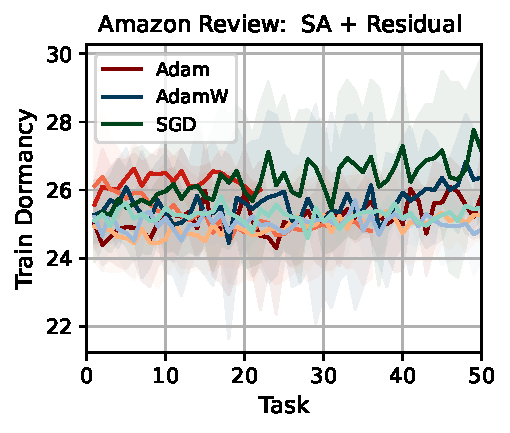
\includegraphics[width=\textwidth]{figs/Accuracy/nlp/transformer_pretrained/amazon_review_full_40.pdf}
        \includegraphics[width=\textwidth]{figs/Accuracy/nlp/transformer_pretrained/yahoo_answers_40.pdf}
        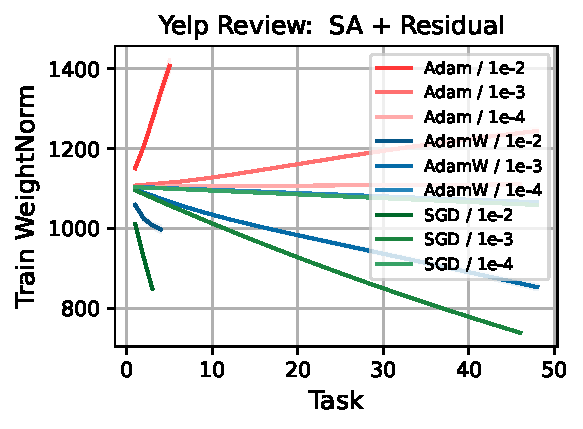
\includegraphics[width=\textwidth]{figs/Accuracy/nlp/transformer_pretrained/yelp_review_full_40.pdf}
        % \includegraphics[width=\textwidth]{figs/Accuracy/nlp/transformer_pretrained/dbpedia_40.pdf}
    }
    % \\
    % \resizebox{\textwidth}{!}{  
    % 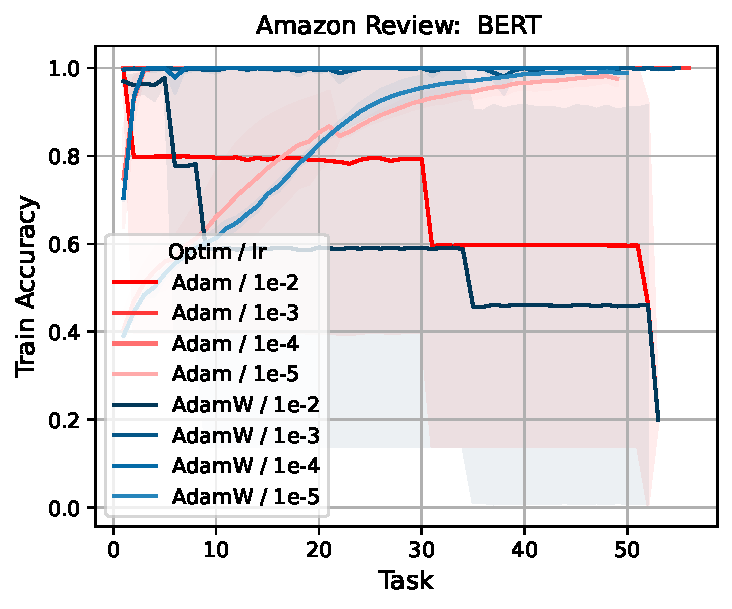
\includegraphics[width=\textwidth]{figs/Accuracy/nlp/bert/amazon_review_full_40.pdf}
    % 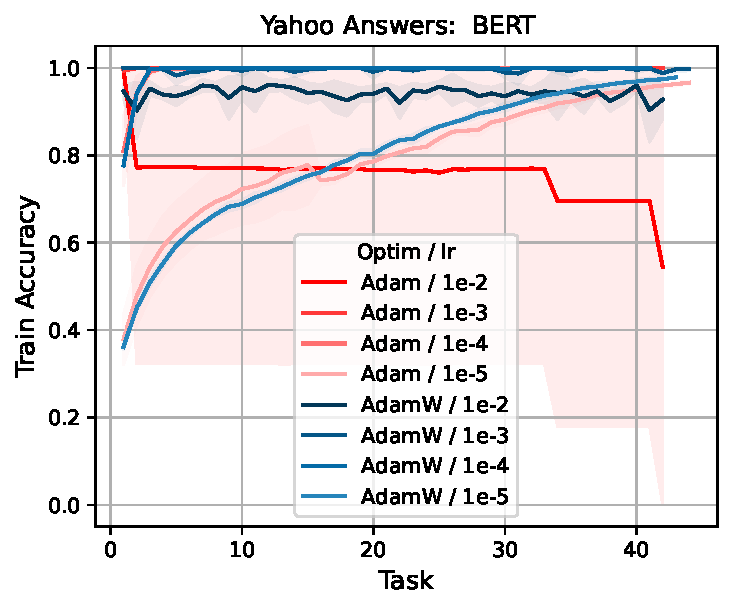
\includegraphics[width=\textwidth]{figs/Accuracy/nlp/bert/yahoo_answers_40.pdf}
    % 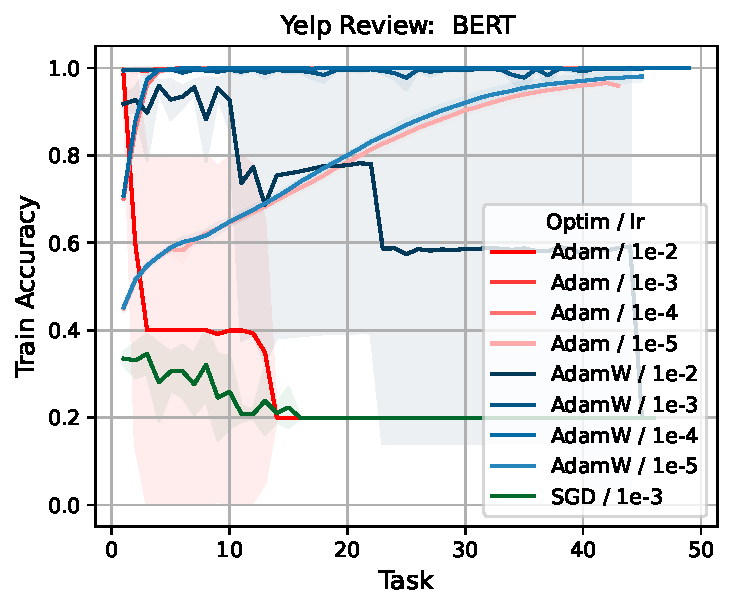
\includegraphics[width=\textwidth]{figs/Accuracy/nlp/bert/yelp_review_full_40.pdf}
    % % 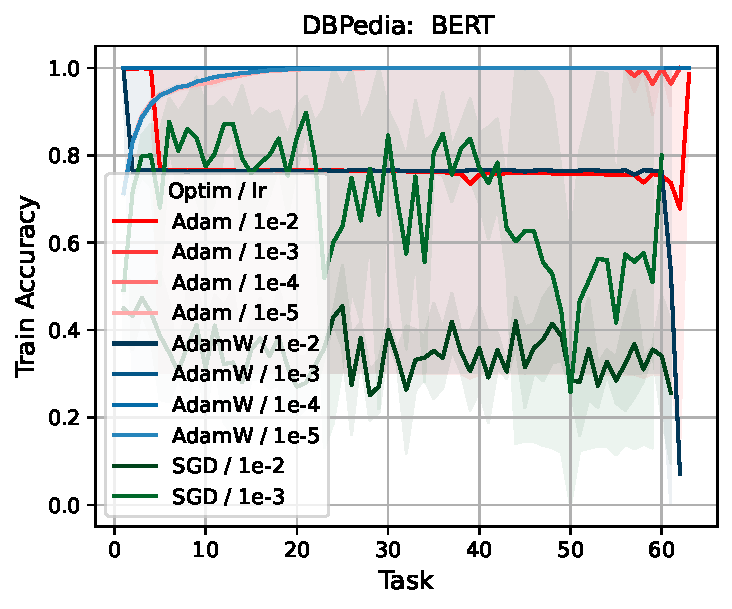
\includegraphics[width=\textwidth]{figs/Accuracy/nlp/bert/dbpedia_40.pdf}
    % }
    \caption{Accuracy of BERT pretrained on NLP datasets.}
    \label{fig:nlp_bert_pretrained}
\end{figure*}


% \subsection{Ablations/Intervention/Analysis}

\subsection{Experiments for other type of networks: MLP, CNN, and LSTM}

To further explore plasticity in NLP datasets, we conducted experiments using various types of networks, including MLP, CNN, and LSTM.

\autoref{fig:nlp_mlp} shows the results of the MLP network for the NLP datasets for both \textit{Individual task-shuffled label} and \textit{Sequential datasets} compared to CIFAR-10. As tasks continue, there is no loss of plasticity for the NLP datasets, whereas there is loss of plasticity for CIFAR-10.


For the CNN experiments with NLP datasets, the network maintains plasticity when using the Adam and AdamW optimizers, but it loses the plasticity with SGD, \autoref{fig:nlp_cnn}. This contrasts with the results for image datasets~\cite{plasticity papers}, as we also demonstrated for CIFAR-10. For image datasets, the network is unable to learn new tasks after a while, even when using Adam and AdamW.

\autoref{fig:nlp_lstm} shows the learning curves for the LSTM network. Both \textit{Individual tasks-shuffled label} and \textit{Sequential datasets} maintain plasticity. Surprisingly, in this case, with CIFAR-10 LSTM also has plasticity and the performance does not decrease. For all cases SGD can not learn the new tasks but Adam and AdamW are able to.

\autoref{fig:nlp_cnn_lstm}



% add ---> \autoref{fig:nlp_mlp} 5 for each data and one for cifar



% \begin{itemize}
%     \item CNN on NLP results. Is there plasticity loss? 
%     \item LSTM on NLP results. Is there plasticity loss? 
% \end{itemize}



% --> mention that we only look at training in this scenario not test or validation and this is different from catastrophic forgetting 

\begin{figure*}[htb!]
    \centering
    \resizebox{\textwidth}{!}{
        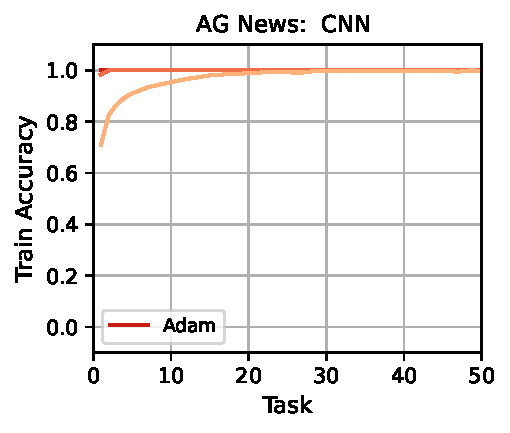
\includegraphics[width=\textwidth]{figs/Accuracy/nlp/cnn/ag_news_50.pdf}
        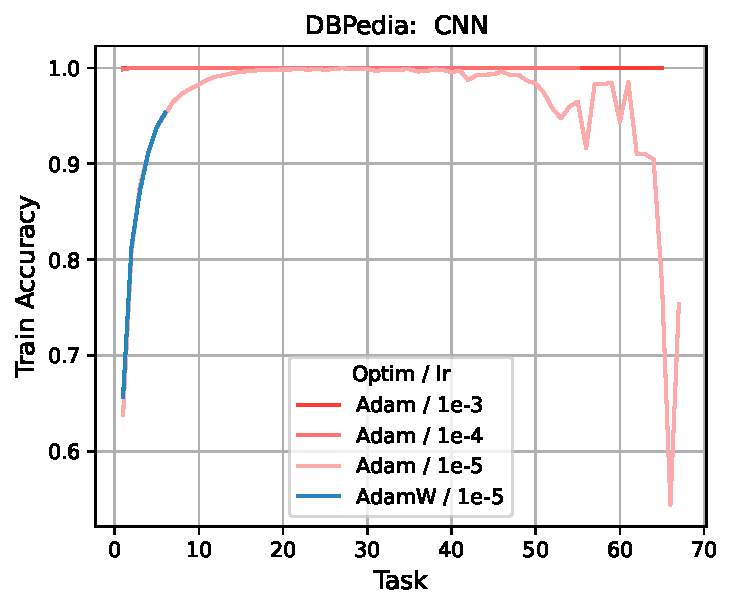
\includegraphics[width=\textwidth]{figs/Accuracy/nlp/cnn/dbpedia_50.pdf}
        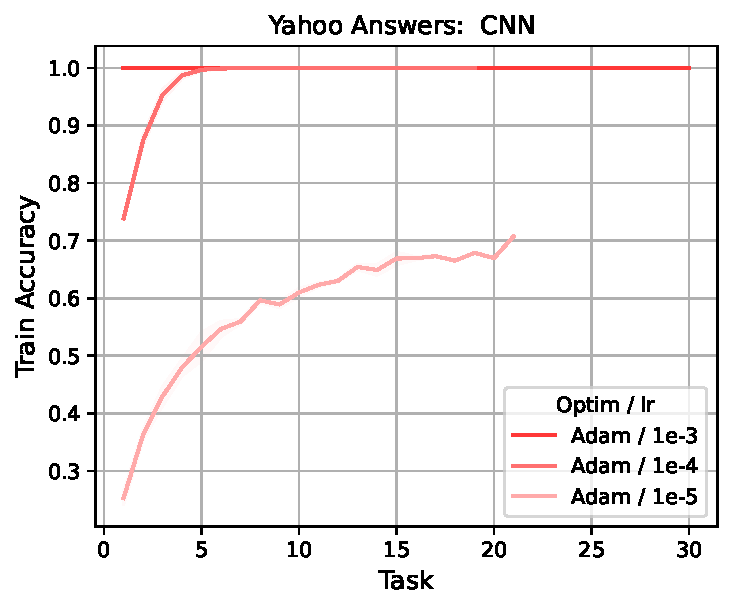
\includegraphics[width=\textwidth]{figs/Accuracy/nlp/cnn/yahoo_answers_50.pdf}
        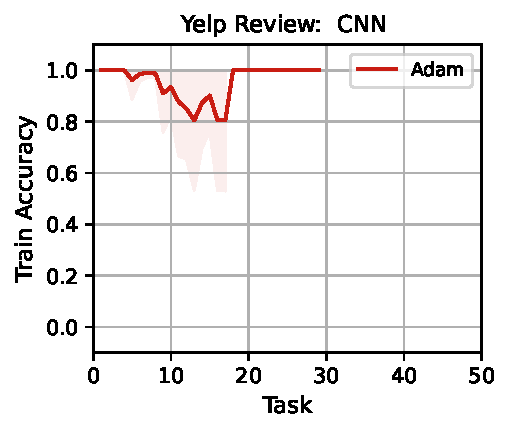
\includegraphics[width=\textwidth]{figs/Accuracy/nlp/cnn/yelp_review_full_50.pdf}
    }
    \\
    \resizebox{\textwidth}{!}{
        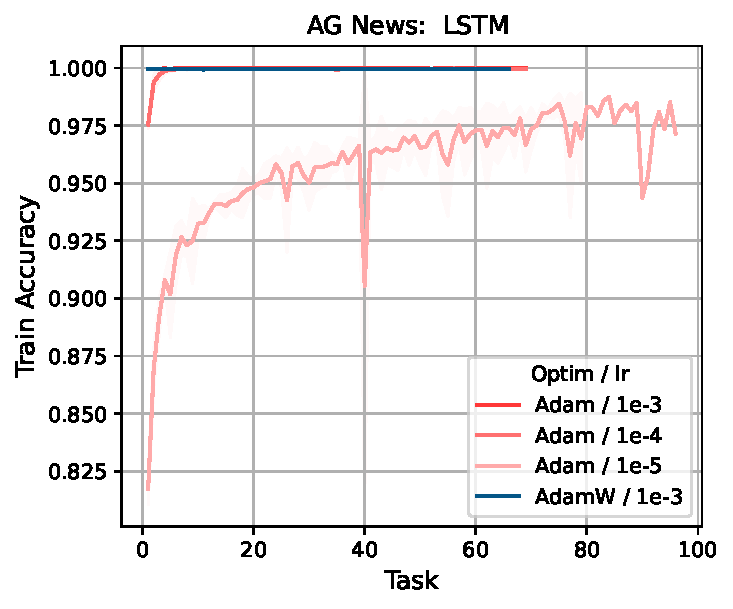
\includegraphics[width=\textwidth]{figs/Accuracy/nlp/lstm/ag_news_50.pdf}
        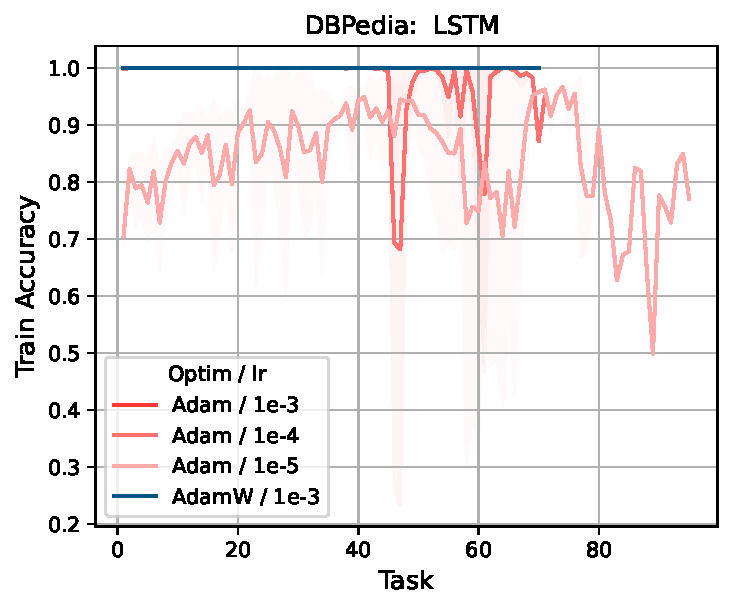
\includegraphics[width=\textwidth]{figs/Accuracy/nlp/lstm/dbpedia_50.pdf}
        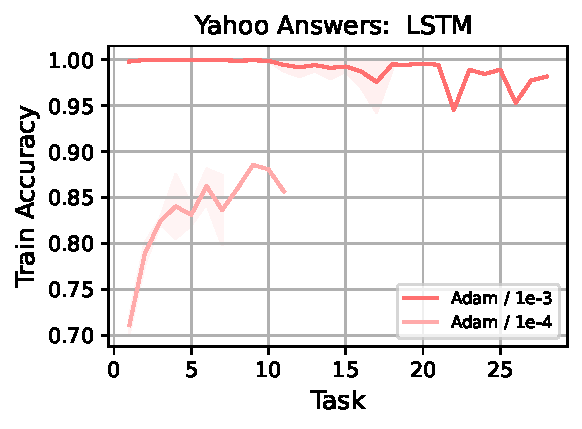
\includegraphics[width=\textwidth]{figs/Accuracy/nlp/lstm/yahoo_answers_50.pdf}
        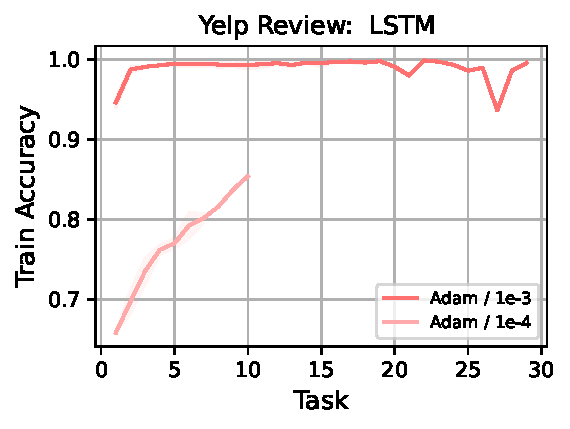
\includegraphics[width=\textwidth]{figs/Accuracy/nlp/lstm/yelp_review_full_50.pdf}
    }
    \caption{Accuracy of CNN and LSTM on NLP datasets.}
    \label{fig:nlp_cnn_lstm}
\end{figure*}

Analysis: \autoref{fig:yahoo_models_analysis}
\begin{figure*}[htb!]
    \centering
    \resizebox{\textwidth}{!}{
        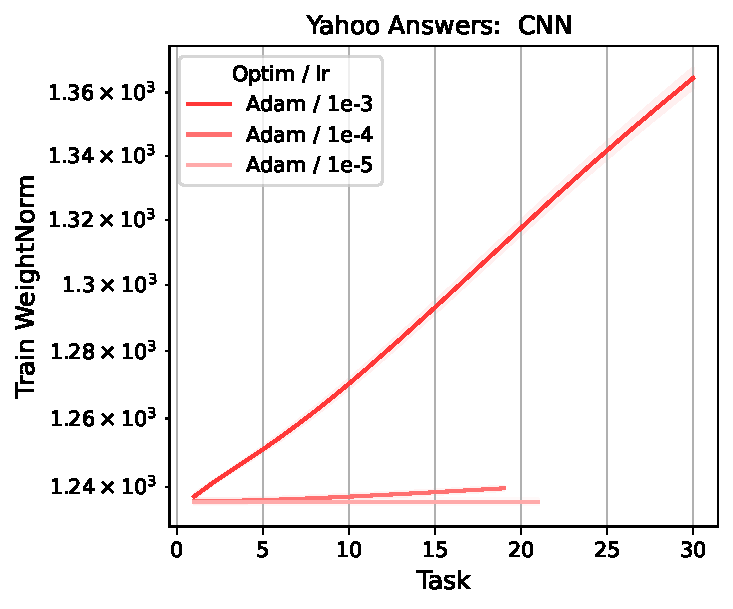
\includegraphics[width=\textwidth]{figs/WeightNorm/nlp/cnn/yahoo_answers_50.pdf}
        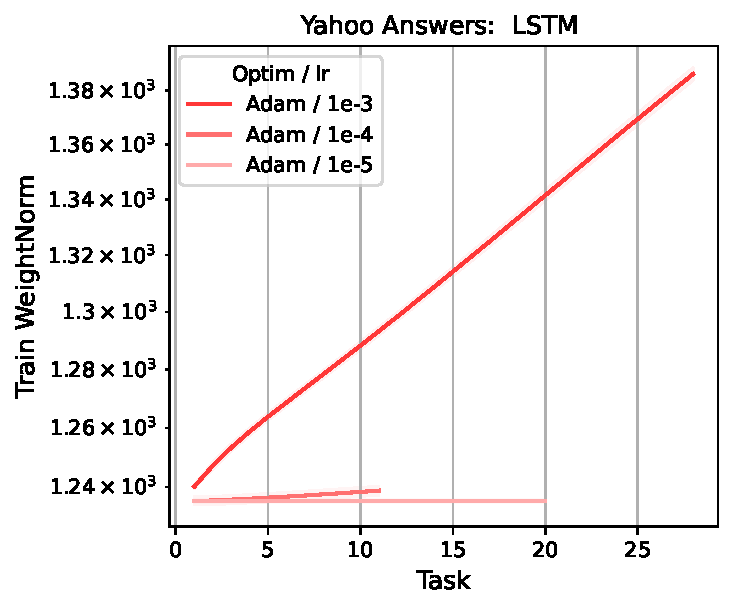
\includegraphics[width=\textwidth]{figs/WeightNorm/nlp/lstm/yahoo_answers_50.pdf}
        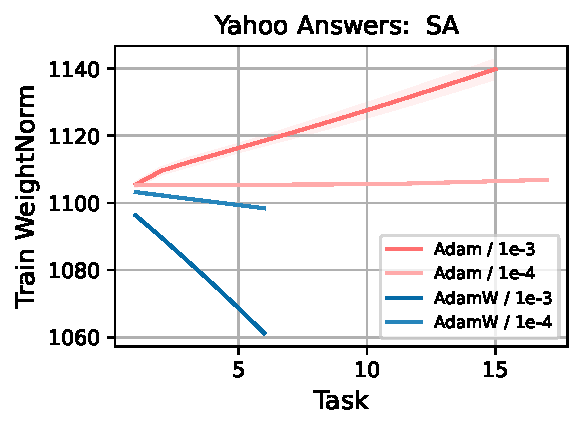
\includegraphics[width=\textwidth]{figs/WeightNorm/nlp/attention/yahoo_answers_40.pdf}
        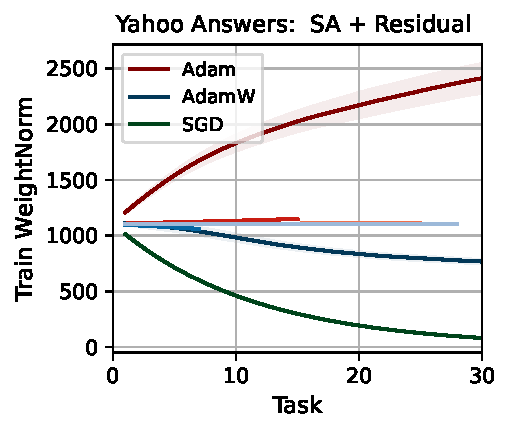
\includegraphics[width=\textwidth]{figs/WeightNorm/nlp/attention_residual/yahoo_answers_40.pdf}
        \includegraphics[width=\textwidth]{figs/WeightNorm/nlp/bert_layer/yahoo_answers_40.pdf}
    }\\    \resizebox{\textwidth}{!}{
        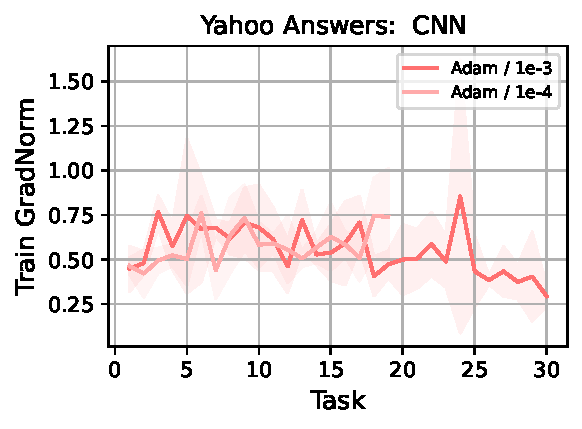
\includegraphics[width=\textwidth]{figs/GradNorm/nlp/cnn/yahoo_answers_50.pdf}
        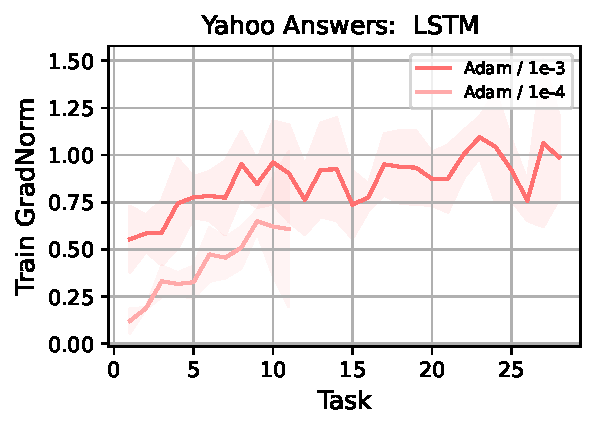
\includegraphics[width=\textwidth]{figs/GradNorm/nlp/lstm/yahoo_answers_50.pdf}
        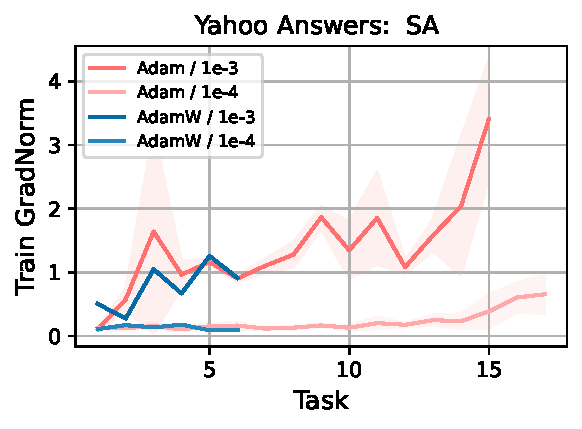
\includegraphics[width=\textwidth]{figs/GradNorm/nlp/attention/yahoo_answers_40.pdf}
        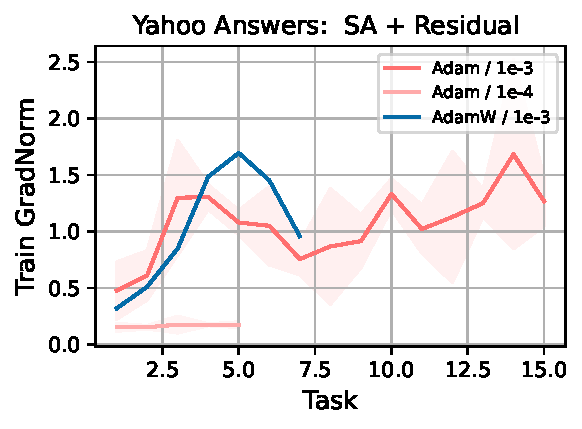
\includegraphics[width=\textwidth]{figs/GradNorm/nlp/attention_residual/yahoo_answers_40.pdf}
        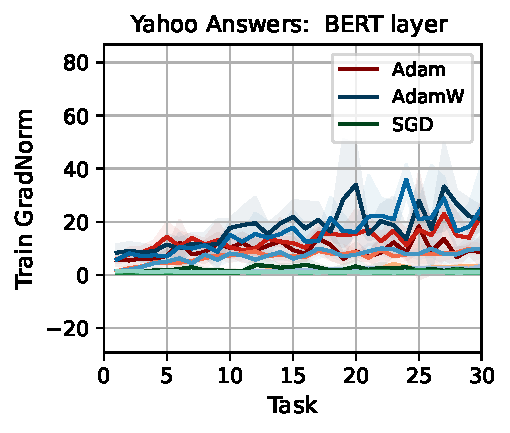
\includegraphics[width=\textwidth]{figs/GradNorm/nlp/bert_layer/yahoo_answers_40.pdf}
    }\\
    \resizebox{\textwidth}{!}{
        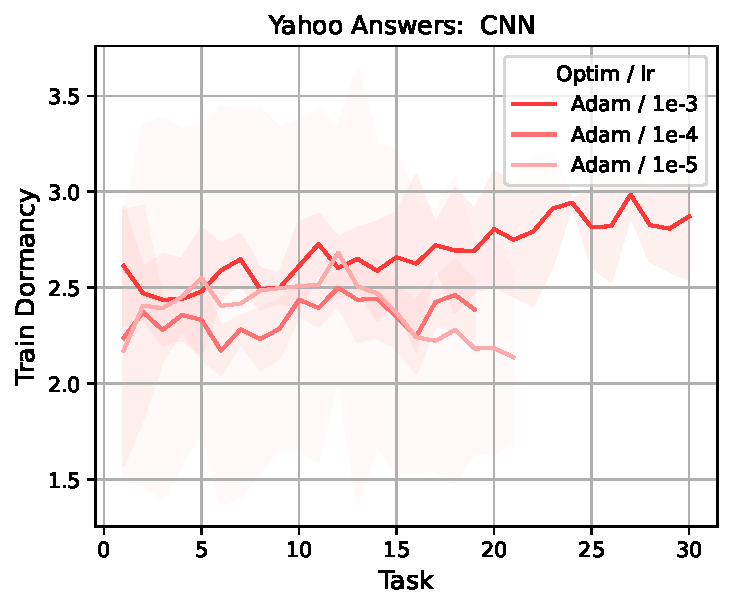
\includegraphics[width=\textwidth]{figs/Dormancy/nlp/cnn/yahoo_answers_50.pdf}
        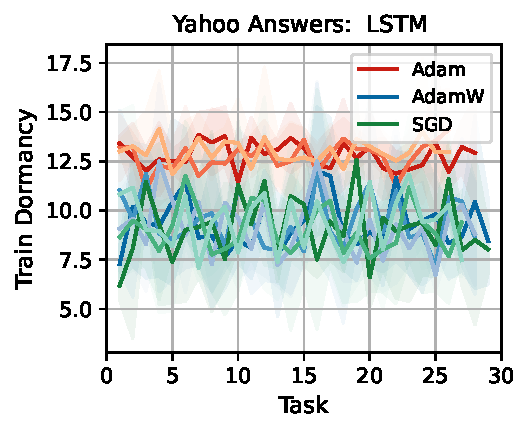
\includegraphics[width=\textwidth]{figs/Dormancy/nlp/lstm/yahoo_answers_50.pdf}
        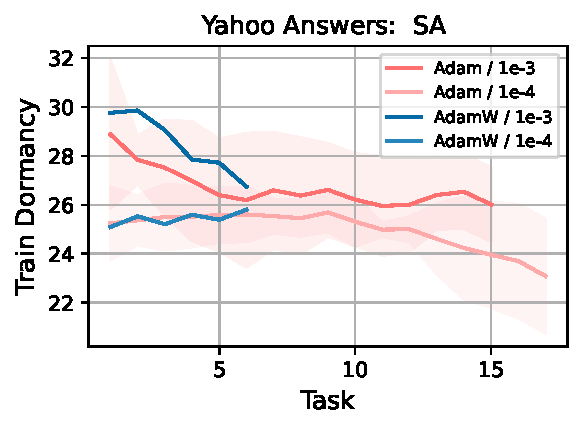
\includegraphics[width=\textwidth]{figs/Dormancy/nlp/attention/yahoo_answers_40.pdf}
        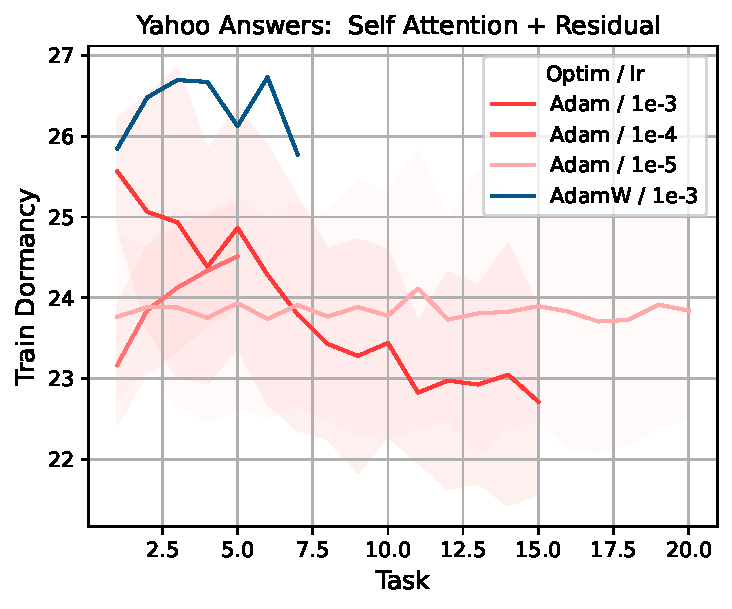
\includegraphics[width=\textwidth]{figs/Dormancy/nlp/attention_residual/yahoo_answers_40.pdf}
        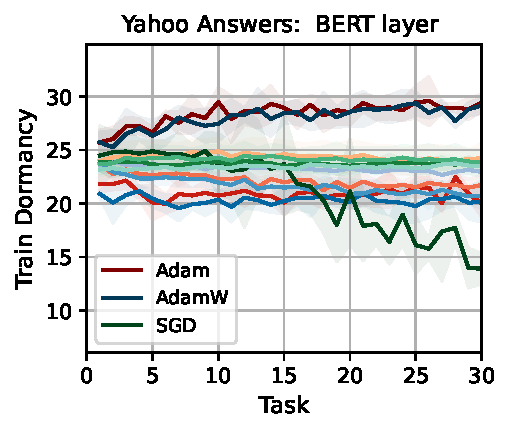
\includegraphics[width=\textwidth]{figs/Dormancy/nlp/bert_layer/yahoo_answers_40.pdf}
    }
    \caption{Analysis of different models on Yahoo Answers datasets.}
    \label{fig:yahoo_models_analysis}
\end{figure*}



\subsection{Comparison with vision}

comparing criteria:
1- we can bring side by side plots from one of the nlp tasks vs image

2- bring sgd vs adam and adamw


\autoref{fig:image_models}
\begin{figure*}[t]
    \centering
    \resizebox{\textwidth}{!}{
        % 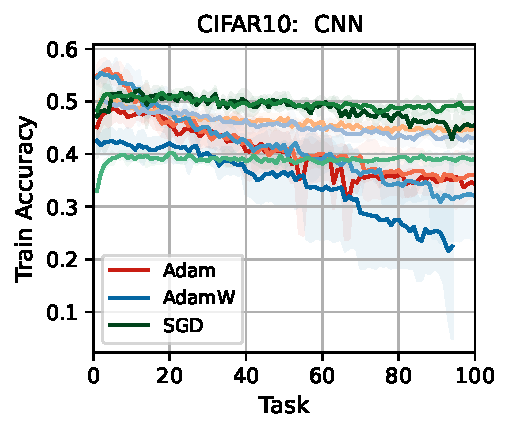
\includegraphics[width=\textwidth]{figs/Accuracy/image/cnn/cifar10_50.pdf}
        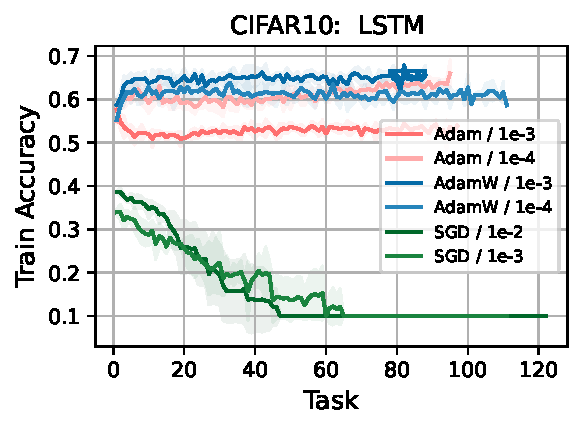
\includegraphics[width=\textwidth]{figs/Accuracy/image/lstm/cifar10_50.pdf}
        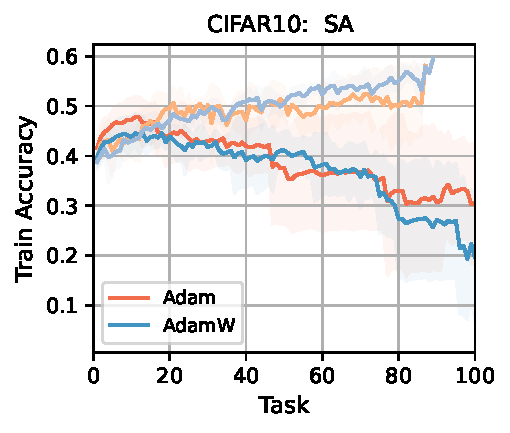
\includegraphics[width=\textwidth]{figs/Accuracy/image/attention/cifar10_40.pdf}
        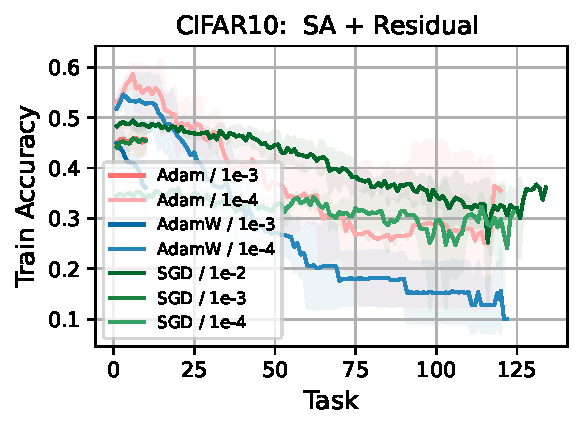
\includegraphics[width=\textwidth]{figs/Accuracy/image/attention_residual/cifar10_40.pdf}
        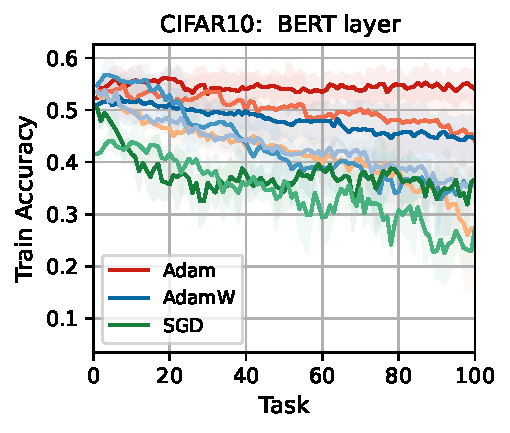
\includegraphics[width=\textwidth]{figs/Accuracy/image/bert_layer/cifar10_40.pdf}
    }
    \caption{Accuracy of different models on CIFAR10.}
    \label{fig:image_models}
\end{figure*}



\subsection{Multi-head-Attention types of the Networks}

In this section, we developed experiments with the networks that have Multi-head Attention layer. The reason was to investigate whether the attention structure will change the plasticity ability. To do so, we designed three type of networks with attention as following:

\autoref{fig:nlp_self_res}

\begin{itemize}
    \item \textit{Multi-head Attention Layer}: the networks comprises of one Embedding, Multi-head Attention layer and one classifier respectively.
    \item \textit{Multi-head Attention Layer with Residual Layer}: the networks is the same as above with a difference that we add input to the output of the attention layer and then feed it to the classifier.
    \item \textit{Bert Layer}: the network is the same as one Bert layer without using any dropout.
\end{itemize}

Note that we considered \textit{Multi-head Attention Layer with Residual Layer} to investigate if a direct stream from input will affect the plasticity.
Also we removed dropout from \textit{Bert Layer} since dropout is one of the solutions to maintain plasticity in images~\cite{}




\begin{figure*}[t]
    \centering
    \resizebox{\textwidth}{!}{
        % 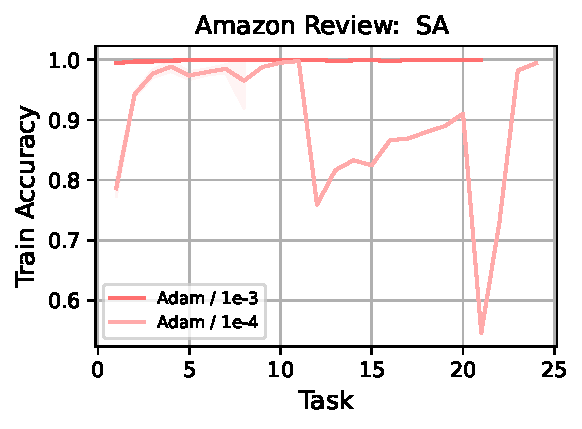
\includegraphics[width=\textwidth]{figs/Accuracy/nlp/attention/amazon_review_full_40.pdf}
        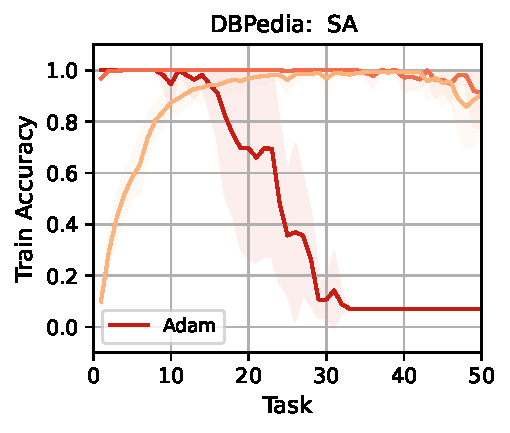
\includegraphics[width=\textwidth]{figs/Accuracy/nlp/attention/dbpedia_40.pdf}
        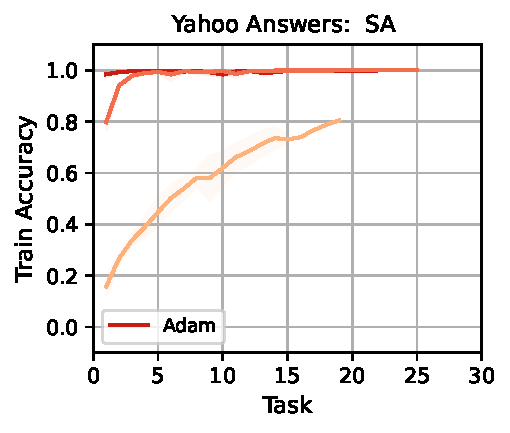
\includegraphics[width=\textwidth]{figs/Accuracy/nlp/attention/yahoo_answers_40.pdf}
        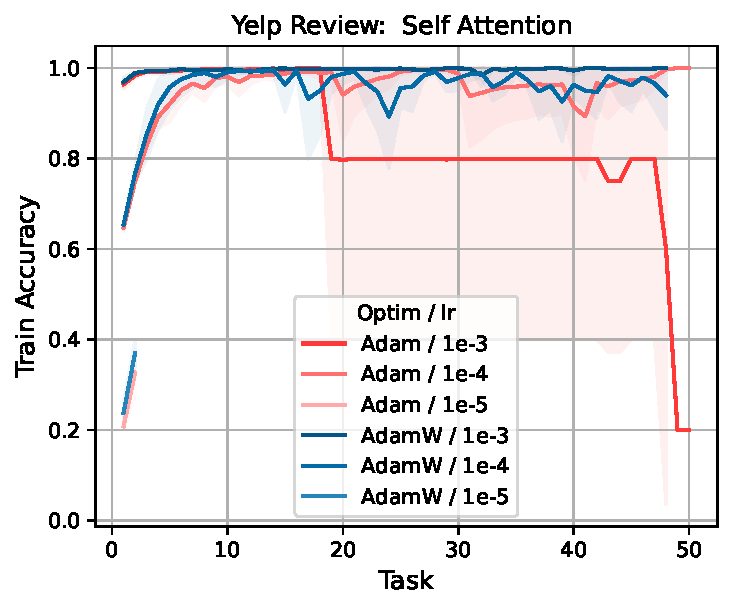
\includegraphics[width=\textwidth]{figs/Accuracy/nlp/attention/yelp_review_full_40.pdf}
    }
    \\
    \resizebox{\textwidth}{!}{
        % 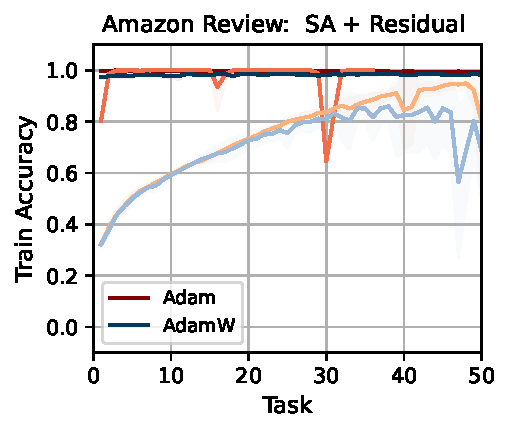
\includegraphics[width=\textwidth]{figs/Accuracy/nlp/attention_residual/amazon_review_full_40.pdf}
        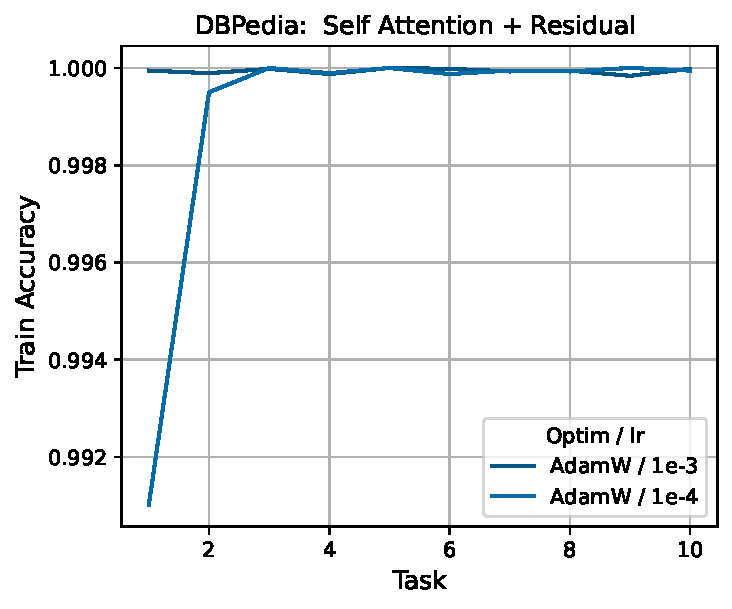
\includegraphics[width=\textwidth]{figs/Accuracy/nlp/attention_residual/dbpedia_40.pdf}
        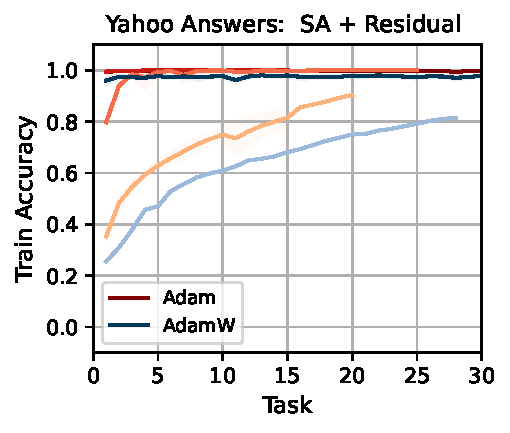
\includegraphics[width=\textwidth]{figs/Accuracy/nlp/attention_residual/yahoo_answers_40.pdf}
        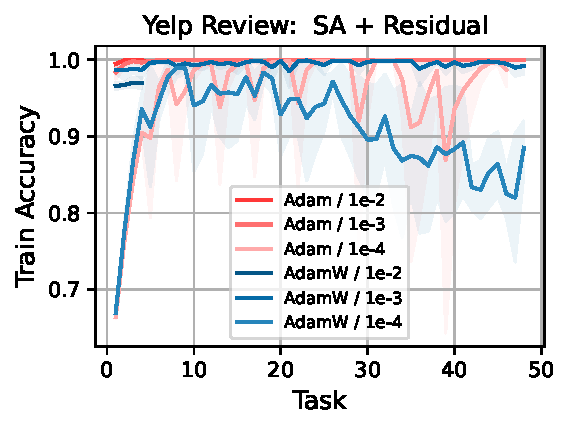
\includegraphics[width=\textwidth]{figs/Accuracy/nlp/attention_residual/yelp_review_full_40.pdf}
    }
    \\
    \resizebox{\textwidth}{!}{
        % 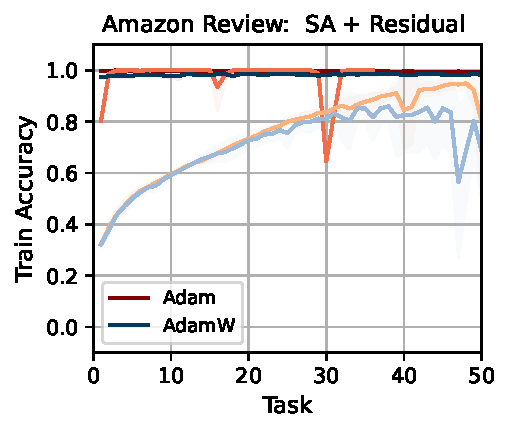
\includegraphics[width=\textwidth]{figs/Accuracy/nlp/attention_residual/amazon_review_full_40.pdf}
        \includegraphics[width=\textwidth]{figs/Accuracy/nlp/bert_layer/dbpedia_40.pdf}
        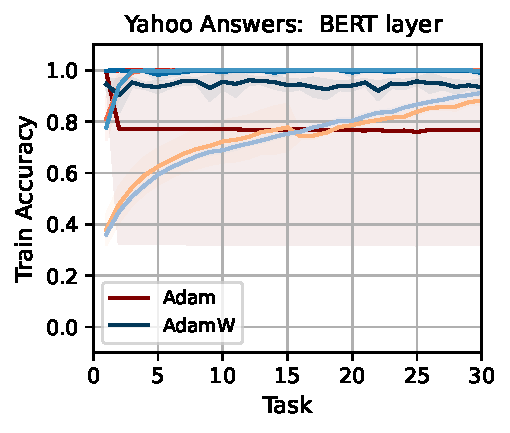
\includegraphics[width=\textwidth]{figs/Accuracy/nlp/bert_layer/yahoo_answers_40.pdf}
        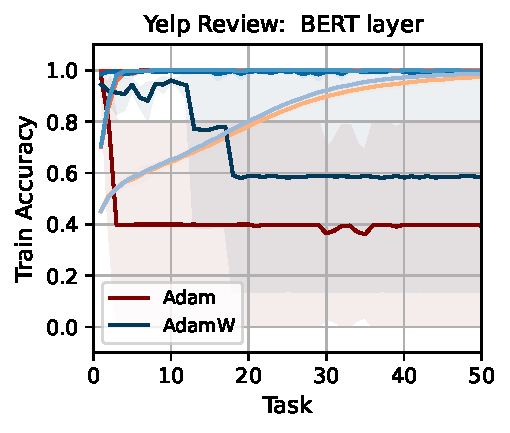
\includegraphics[width=\textwidth]{figs/Accuracy/nlp/bert_layer/yelp_review_full_40.pdf}
    }

    \caption{Accuracy of Self attenstion, Self attenstion with residual layer, and one BERT layer on NLP datasets.}
    \label{fig:nlp_self_res}
\end{figure*}


\subsection{Data distributions}
\autoref{fig:5nlp_models}

\begin{figure*}[t]
    \centering
    \resizebox{\textwidth}{!}{
        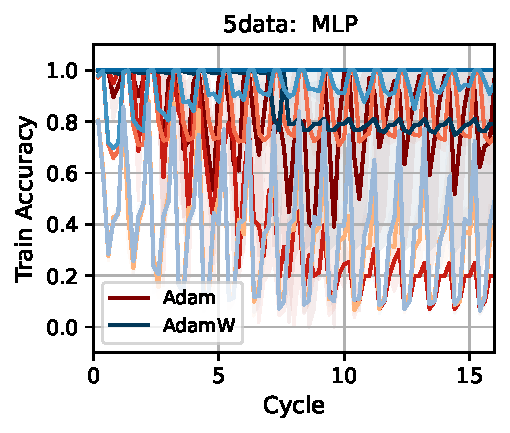
\includegraphics[width=\textwidth]{figs/Accuracy/5nlp/mlp/5data_50.pdf}
        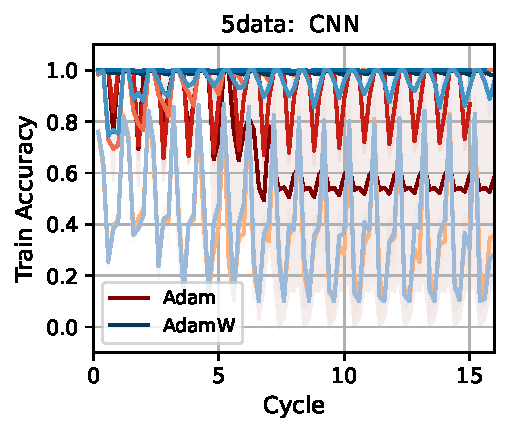
\includegraphics[width=\textwidth]{figs/Accuracy/5nlp/cnn/5data_50.pdf}
        \includegraphics[width=\textwidth]{figs/Accuracy/5nlp/lstm/5data_50.pdf}
    }\\
    \resizebox{\textwidth}{!}{
        \includegraphics[width=\textwidth]{figs/Accuracy/5nlp/attention/5data_40.pdf}
        \includegraphics[width=\textwidth]{figs/Accuracy/5nlp/attention_residual/5data_40.pdf}
        \includegraphics[width=\textwidth]{figs/Accuracy/5nlp/bert_layer/5data_40.pdf}
    }
    \caption{Accuracy of different models on 5 NLP dataset.}
    \label{fig:5nlp_models}
\end{figure*}






\section{Discussion and Future Works}


\section{Conclusion}
% \subsection{Plasticity in NLP}
% \subsection{Plasticity in self-attention networks}
% Bibliography entries for the entire Anthology, followed by custom entries
%\bibliography{anthology,custom}
% Custom bibliography entries only
\bibliography{custom}
\appendix
\section{Example Appendix}
\label{sec:appendix}

This is an appendix.


\end{document}
